\section{Partial correlation}

\subsection{Definition of partial correlation}

\marginnote{
Partial correlation is a~measure of degree of dependence between two random
variables while controlling for the~effect of other random variables:
\[
\pCorr(X,Y; Z) = \frac{\pCov(X,Y;Z)}{\sqrt{\pVar(X;Z)\pVar(Y;Z)}}
\]
where $\pVar(X;Z) = \Var(X - \alpha Z)$, $\alpha$ is such a~constant that $\Cov(X - \alpha Z, Z) = 0$,
and $\pCov(X,Y; Z) = \Cov(X - \alpha Z, Y - \beta Z)$, $\alpha$, $\beta$ are such
constants that $\Cov(X - \alpha Z, Z) = \Cov(Y - \beta Z, Z) = 0$.
}

Partial correlation can be defined in two ways.
We will provide both definitions and show their equivalence.

\begin{definition}
Partial correlation between random variables $X$ and $Y$ holding random variable $Z$
fixed is the~correlation coefficient between the~residuals in regression of $X$ onto
$Z$ and the~residuals in regression of $Y$ onto $Z$.
\end{definition}

Firstly, we project random variable $X$ onto $Z$, which yields $\E(X \vert Z)$.
The residuals in this regression are $X - \E(X \vert Z)$ — a vector in $Lin^{\perp}(Z)$.
We will call this variable `cleansed' and label it as $\widetilde X$.
Applying the same procedure for $Y$ yields `cleansed' variable $\tilde Y = Y - \E(Y \vert Z) \in Lin^{\perp}(Z)$.
The~angle between $\widetilde X$ and $\widetilde Y$ ($\varphi$ in Figure~\ref{fig:pcorr_def1})
is the~correaletion coefficient between these `cleansed' random variables and
the~partial correlaiton between the~original ones.

\begin{figure}
\centering
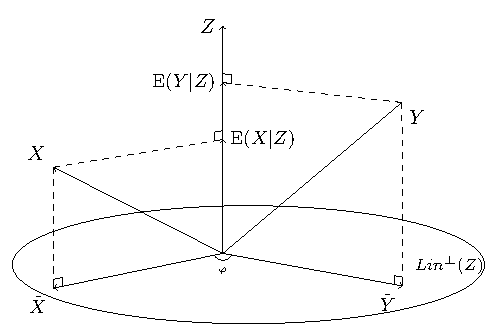
\includegraphics[width=0.55\linewidth]{figures/03_partial_correlation_definition.pdf}
\caption{Partial correlation between $X$ and $Y$ while $Z$ is fixed.}
\label{fig:pcorr_def1}
\end{figure}

\marginnote{
Let us define $\widetilde X$ and $\widetilde Y$ as
\begin{align*}
\widetilde X &= \alpha_{XY} \widetilde Y + \tilde{u}_{XY}, \widetilde X \perp Z \\
\widetilde Y &= \alpha_{YX} \widetilde X + \tilde{u}_{YX}, \widetilde Y \perp Z
\end{align*}
Then assuming that the~error term $u_{XY}$ is uncorrelated with $\widetilde Y$,
we obtain:
\begin{align*}
&\Cov(\widetilde Y, \widetilde X - \alpha_{XY} \widetilde Y) = 0 \\
&\Cov(\widetilde Y, \widetilde X) - \alpha_{XY} \Cov(\widetilde Y, \widetilde Y) = 0 \\
&\alpha_{XY} = \frac{\Cov(\widetilde Y, \widetilde X)}{\Var(\widetilde Y)}
\end{align*}
In the same manner we get $\alpha_{YX}$:
\[
\alpha_{YX} = \frac{\Cov(\widetilde Y, \widetilde X)}{\Var(\widetilde X)}
\]
Note, that $\alpha_{XY}$ and $\alpha_{XY}$ are of the~same sign.
}

\begin{definition}
Partial correlaiton between random variables $X$ and $Y$ holding random variable $Z$
fixed is the~geometric mean between the coefficient $\beta_{XY}$ in regression
\[
X = \beta_{XY} Y + \beta_{XZ} Z + u_X
\]
and the~coefficinent $\beta_{YX}$ in regression
\[
Y = \beta_{YX} X + \beta_{YZ} Z + u_Y
\]
Partial correlation has the same sign as the~coefficients $\beta_{XY}$ and $\beta_{YX}$.
\end{definition}

Following the~definition, we need to start with regressing variable $X$ onto
$Y$ and $Z$. Then, the vector we obtain $\hat X = \E(X \vert Y, Z)$
can be broken up into the sum of $\beta_{XY} Y$ and $\beta_{XZ} Z$.
Projecting $\beta_{XY} Y$ onto $Lin^{\perp}(Z)$ results in a~vector
$\alpha_{XY} \widetilde Y$ where $\widetilde Y = Y - \E(Y \vert Z)$
is the projection of $Y$ onto $Lin^{\perp}(Z)$.

\marginnote{
Multiplying these coefficients, we get the final result:
\begin{multline*}
\alpha_{XY} \cdot \alpha_{XY} = \frac{\Cov^2(\widetilde Y, \widetilde X)}{\Var(\widetilde Y)\Var)\widetilde X} \\
= \Corr^2(\widetilde X, \widetilde Y) = \pCorr^2(X,Y; Z)
\end{multline*}
}

By the~properties of similar triangles
\[
\frac{\beta_{XY} Y}{Y} = \frac{\alpha_{XY} \widetilde Y}{\widetilde Y} \Leftrightarrow \beta_{XY} = \alpha_{XY}
\]

In the same way we perform a regression of $Y$ onto $X$ and $Z$ and repeat the
same steps for $X$. Finally, we get the whole picture:

\begin{figure}[ht!]
\begin{center}
\subfigure[]{
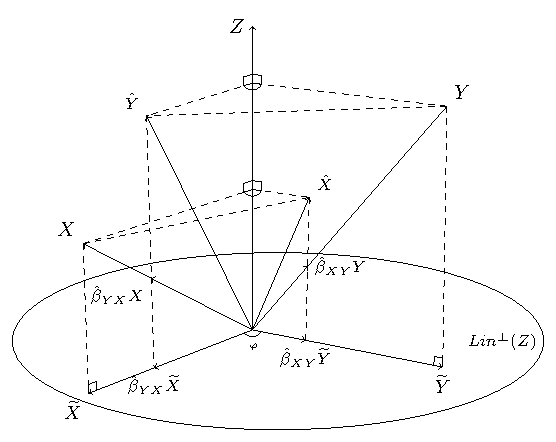
\includegraphics[width=0.55\linewidth]{figures/03_partial_correlation_regression_definition.pdf}
\label{fig:part_corr_alt}}
\subfigure[]{
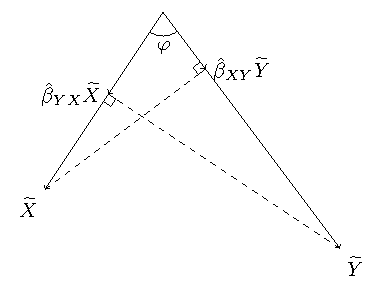
\includegraphics[width=0.35\linewidth]{figures/03_partial_correlation_regression_definition_lin.pdf}
\label{fig:part_corr_alt_lin}}
\caption{\subref{fig:part_corr_alt}: Alternative definition of the partial correlation;
\subref{fig:part_corr_alt_lin}: $Lin^{\perp}(Z)$.}
\end{center}
\end{figure}

Having plotted $Lin^{\perp}(Z)$, now we can express $\cos \varphi$ in terms of $\beta_{XY}$
and $\beta_{YX}$:

\begin{equation*}%\label{eq:part_cor_cos}
\begin{split}
\cos \varphi &= \frac{\vert \beta_{XY} \widetilde Y \vert}{\vert \widetilde X \vert} \\
\cos \varphi &= \frac{\vert \beta_{YX} \widetilde X \vert}{\vert \widetilde Y \vert} \\
\cos^2 \varphi &= \vert \beta_{XY} \beta_{YX} \vert \stackrel{\beta_{XY} \beta_{YX} > 0}{=} \beta_{XY} \beta_{YX}
\end{split}
\end{equation*}

Recall that the angle $\varphi$ can be interpreted as the correlation
between $\widetilde X$ and $\widetilde Y$.
These random variables are constructed in such a way that both of them
are uncorrelated with $Z$. Thus, it follows that
\[
\cos^2 \varphi = \Corr^2(\widetilde X, \widetilde Y) = \pCorr^2(X,Y; Z) = \beta_{XY} \beta_{YX}
\]

\subsection{Partial correlation as correlaiton between residuals}

\marginnote{
Let us define cleansed $X$ and $Y$ first as
\begin{align*}
\widetilde{X} &= \alpha_1 \widetilde{Y} + \tilde{u}, \widetilde{X} \perp Z \\
\widetilde{Y} &= \beta_1 \widetilde{X} + \tilde{v}, \widetilde{Y} \perp Z
\end{align*}
Then
\begin{align*}
\alpha_1 &= \frac{\Cov(\widetilde{X}, \widetilde{Y})}{\Var(\widetilde{Y})} \\
\beta_1 &= \frac{\Cov(\widetilde{X}, \widetilde{Y})}{\Var(\widetilde{X})}
\end{align*}
}



\begin{theorem}
Partial correlaiton between $X$ and $Y$ holding $Z$ fixed is the negative
correlaiton coefficient betwenn the residuals $u$ in the regeression model
\[
X = \alpha_1 Y + \alpha_2 Z + u
\]
and the residuals $v$ in the model
\[
Y = \beta_1 X + \beta_2 Z + v
\]
\end{theorem}

\begin{proof}
The first step is to find the residuals in the mentioned regresisions.
For example, in order to get $u$ we regress $X$ onto $Lin(Y,Z)$
which results in $\hat X = X - \E(X \vert Y, Z)$.
Then we take the difference $X - \hat X = u$
and project it as well as $X$ itself onto $Lin^{\perp}(Z)$ as demonstrated
in Figure~\ref{fig:pcorr_t_x}.
We denote the result as $\tilde u$ and $\widetilde X$ respectively.

\marginnote{
Substituting these into $\Cov(\tilde{u}, \tilde{v})$, we obtain:
\begin{align*}
&\Cov(\tilde{u}, \tilde{v}) = \\
&\Cov\left(\widetilde{X} - \frac{\Cov(\widetilde{X}, \widetilde{Y})}{\Var(\widetilde{Y})} \widetilde{Y},
\widetilde{Y} -  \frac{\Cov(\widetilde{X}, \widetilde{Y})}{\Var(\widetilde{X})} \widetilde{X}\right) \\
&= \Cov(\widetilde{X}, \widetilde{Y}) - \Cov(\widetilde{X}, \widetilde{Y}) \\
&- \Cov(\widetilde{X}, \widetilde{Y}) + \frac{\Cov^3(\widetilde{X}, \widetilde{Y})}{\Var(\widetilde{X})\Var(\widetilde{Y})} \\
&= - \Cov(\widetilde{X}, \widetilde{Y}) \left(1 - \frac{\Cov^2(\widetilde{X}, \widetilde{Y})}{\Var(\widetilde{X})\Var(\widetilde{Y})} \right)
\end{align*}
Next, we deal with variances of $\tilde{u}$ and $\tilde{v}$:
\begin{align*}
&\Var(\tilde{u}) = \Var(\widetilde{X}) - \frac{\Cov^2(\widetilde{X}, \widetilde{Y})}{\Var^2(\widetilde{Y})} \Var(\widetilde{Y}) \\
&- 2 \Cov(\widetilde{X}, \widetilde{Y}) \frac{\Cov(\widetilde{X}, \widetilde{Y})}{\Var(\widetilde{Y})} \\
&= \Var(\widetilde{X}) \left(1 - \frac{\Cov^2(\widetilde{X}, \widetilde{Y}}{\Var(\widetilde{X}) \Var(\widetilde{Y})}\right) \\
&\Var(\tilde{v}) = \Var(\widetilde{Y}) \left(1 - \frac{\Cov^2(\widetilde{X}, \widetilde{Y}}{\Var(\widetilde{X}) \Var(\widetilde{Y})}\right)
\end{align*}
Now we can write out $\Corr(\tilde{u}, \tilde{v})$:
\begin{align*}
&\Corr(\tilde{u}, \tilde{v}) = \\
&= -\frac{\Cov(\widetilde{X}, \widetilde{Y}) \left(1 - \frac{\Cov^2(\widetilde{X}, \widetilde{Y})}{\Var(\widetilde{X})\Var(\widetilde{Y})} \right)}{\sqrt{\Var(\widetilde{X})\Var(\widetilde{Y}) \left(1 - \frac{\Cov^2(\widetilde{X}, \widetilde{Y})}{\Var(\widetilde{X}) \Var(\widetilde{Y})}\right)^2 }} \\
&= -\Corr(\widetilde{X}, \widetilde{Y})
\end{align*}
}

Figure~\ref{fig:pcorr_t_y} shows the same steps for obtainig $\tilde v$ and $\widetilde Y$.

\begin{figure}[ht!]
\begin{center}
\subfigure[]{
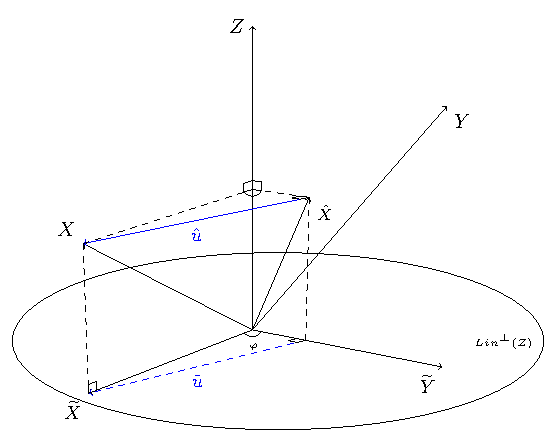
\includegraphics[width=0.45\linewidth]{figures/03_partial_correlation_residuals_x.pdf}
\label{fig:pcorr_t_x}}
\subfigure[]{
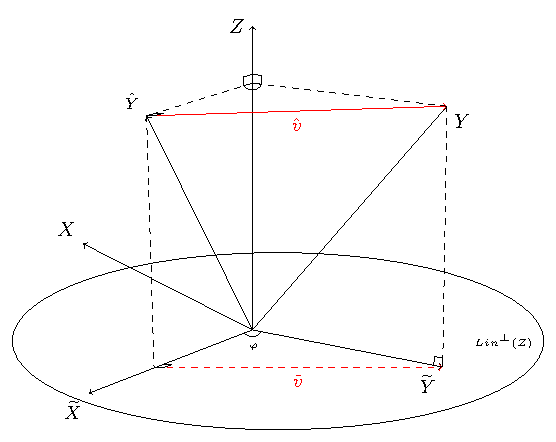
\includegraphics[width=0.45\linewidth]{figures/03_partial_correlation_residuals_y.pdf}
\label{fig:pcorr_t_y}}
\caption{\subref{fig:pcorr_t_x}: $\hat u$ form regression of x onto $Y$ and $Z$, $\hat u$ projected;
\subref{fig:pcorr_t_y}: $\hat v$ from regression of $Y$ onto $X$ and $Z$, $\hat v$ projected.}
\setfloatalignment{b}
\end{center}
\end{figure}



After putting these figures together, we need to measure the angle
between the $\tilde u$ and $\tilde v$.
Translating the $\tilde v$ vector to the orgin of $\tilde x$ as shown in Figure~\ref{fig:pcorr_t_lin},
we conclude that the desired angle is the bigger one of the vertical angles.
Hence, we can derive it from the property of quadrilateral
by substracrtion all the known angles from $360^\circ$.
Thus, the desired one is equal to $180^\circ - \varphi$.
\begin{align*}
\cos(\varphi) &= - \cos(180^\circ - \varphi) \\
\Corr(\widetilde X, \widetilde Y) &= -\Corr(\tilde u, \tilde v) \\
\pCorr(X,Y; Z) &= -\Corr(u, v)
\end{align*}


\begin{figure}[ht!]
\begin{center}
\subfigure[]{
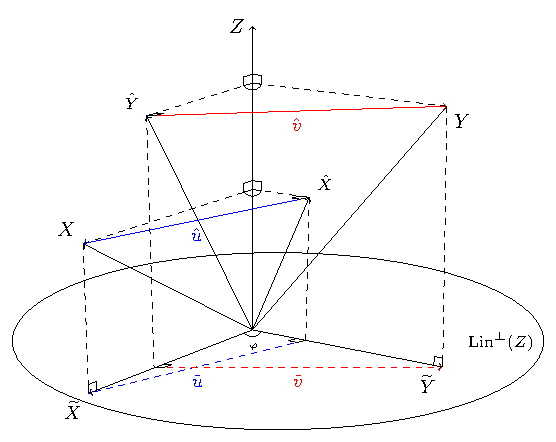
\includegraphics[width=0.45\linewidth]{figures/03_partial_correlation_residuals_xy.pdf}
\label{fig:pcorr_t_xy}}
\subfigure[]{
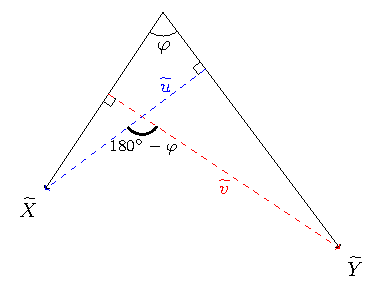
\includegraphics[width=0.45\linewidth]{figures/03_partial_correlation_residuals_xy_lin.pdf}
\label{fig:pcorr_t_lin}}
\caption{\subref{fig:pcorr_t_x}: The residuals of both regressions;
\subref{fig:pcorr_t_y}: $Lin^{\perp}(Z)$.}
\setfloatalignment{b}
\end{center}
\end{figure}
\end{proof}
